\section{Internet-scale analysis}
\label{sec:internet-scale}

We now explore how effective \name attacks might be in practice by modeling
the activity of Tor users, emulating the corresponding Tor path
selection of these users, and inferring the prevalence of AS-level
adversaries who have the ability to mount the attacks that we described
in the preceding sections.

\subsection{Approach}

We aim to quantify the likelihood that an AS will be able to mount a
\name attack.  Figure~\ref{fig:simulations} summarizes our simulation approach,
which we detail in the next section. In short, we model the activity of Tor users
and simulate corresponding Tor path selection using TorPS~\cite{TorPS}.
TorPS returns guard and exit relays, which we then feed as
input---together with source ASes and destination addresses---into our
framework that runs traceroutes from RIPE Atlas nodes.  The rest of this
section describes our approach in detail.

\subsubsection{Attack model}

\begin{figure}[t]
	\centering
	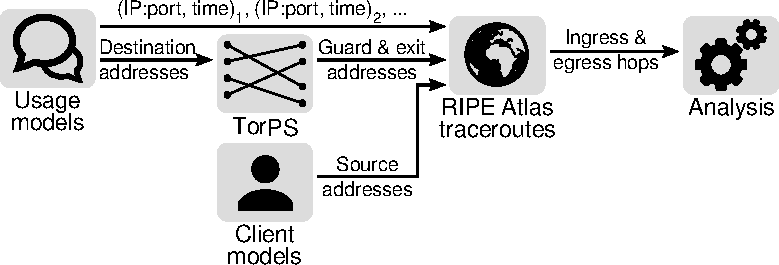
\includegraphics[width=\linewidth]{figures/simulations.pdf}
	\caption{The relation among our simulation components.  Our goal is to
	determine the ASes a Tor user's traffic traverses into and out of the Tor
	network.  Duplicate ASes on both sides can deanonymize streams.}
	\label{fig:simulations}
\end{figure}


We assume that an AS that can see both traffic entering the Tor network 
and DNS traffic exiting the Tor network for the purposes of mounting
a \name attack. 
A Tor exit can perform DNS resolution in two ways: \first~running a name server
locally; \second~or relying on a third-party name server, such as its ISP's name
server or a public DNS name server such as Google's open public DNS
resolver.  In the case of Tor
exits that perform local DNS resolution, an effective position for an attacker
is both \first~anywhere on the AS path between a Tor client and its
guard relay; and \second~anywhere on the path between a Tor exit and any of the
name servers the exit has to communicate with to resolve the name.
These name servers include the root name servers and subsequent name servers in
the DNS hierarchy.  All ASes along the path from the exit relay
to the name servers will be able to see the domain names that the exit
relay is querying.
For Tor exits that rely on third-party DNS resolvers, the
adversary instead has to be on the path between the exit relay and its DNS
resolver.
%)\fixme{QUESTION: ``In addition, the DNS queries will look like they are coming
%from the IP address of the name server and not the IP address of the
%exit relay.''--This new wording seems unclear to me now--wanted to say 
%that ASes on the path from the 3rd-party to the DNS servers will see that 
%the queries are coming from the 3rd-party and not the exit IP, which is 
%why we ignore them . . .}

\subsubsection{Simulating Tor user activity with TorPS}

To measure the likelihood that an AS can be in a position to perform a \name
attack, we use TorPS, the Tor Path Simulator, which mimics how the Tor client
software constructs circuits~\cite{TorPS}.  TorPS takes as input archived Tor
network data~\cite{collector} and usage models, which are basically sets of IP
addresses that Tor clients talk to---\eg web servers.  Given this input, TorPS
then simulates for a configurable number of ``virtual'' Tor clients the way they
would select guard and exit relays.  TorPS is based on the Tor stable release in
version 0.2.4.23.  For each simulated client, TorPS uses one guard; this guard
selection expires after 270 days. We use TorPS to emulate the behavior of
100,000 Tor clients for the entire month of March 2016.

% \fixme{Wording, please: ``we perform 100,000 samples in the TorPS Monte Carlo 
% simulation'' or ``we perform 100,000 Monte Carlo simulations in order to 
% analyze this.''}
%potential Tor users and how the Tor client would have behaved.
%we perform 100,000 samples in the TorPS Monte Carlo
%simulation.  

For the Internet-scale analysis, we also need to place simulated Tor clients
into an AS.  We selected clients in major ISPs in the top-five most popular
countries of Tor usage according to Tor Metrics.\footnote{URL available at
\url{https://metrics.torproject.org/userstats-relay-table.html}.} As of August
2016, the top five countries are the U.S., Russia, Germany, France, and the U.K.
For the U.S., we chose Comcast (AS~7922); for Russia, Rostelecom (AS~42610); for
Germany, Deutsche Telekom (AS~3320); for France, Orange (AS~3215); and for Great
Britain, British Telecom (AS~2856).

Having placed simulated Tor clients into ASes, we now determine their activity
over Tor.  We model each client to have visited several websites every day in March 2016.  We
modeled our client behavior off of the ``Typical'' model used
by Johnson et al.~\cite[\S~5.1.2]{Johnson2013a}.  At 9 a.m. EST, the client visits
{\tt mail.google.com} and {\tt www.twitter.com}.  At 12 p.m. EST, the client visits
{\tt calendar.google.com} and {\tt docs.google.com} 
At 3 p.m. EST, the client visits {\tt www.facebook.com} and {\tt www.instagram.com}. 
Finally, at 6 p.m. EST the client 
visits {\tt www.google.com}, {\tt www.startpage.com}, and {\tt www.ixquick.com}, 
and at 6:20 p.m. EST the client visits {\tt www.google.com}, {\tt www.startpage.com}, 
and {\tt www.ixquick.com} again. Each of the 100,000 simulated Tor clients thus
had 372 opportunities to be compromised given 31 days and 12 site visits per
day.  TorPS provided a new circuit every ten minutes, regardless of how many
distinct connections the client made to different sites; it did not provide a
new circuit for different websites if the client visited the group of sites
within the same ten-minute window.
% This behavior differs from the latest Tor
% Browser, which provides new circuit for each distinct website, even within the
% same ten-minute time interval.  Thus, our results will be conservative in this
% respect.

For simplicity, we assume that only one DNS request occurs every time the client
visits a site. For example, in our model, at 9 a.m. one DNS request will occur
for {\tt mail.google.com} and one DNS request will occur for {\tt
www.twitter.com}. At 6 p.m. three DNS requests will occur, and at 6:20 p.m.
those same three DNS requests will occur again.   For now, we do
not take embedded requests or caching into account.
%\xxx{Shouldn't each
%  website actually result in hundreds of DNS lookups? This process could
%be more clear.} 

\subsubsection{Inferring AS-level paths: traceroute + {\tt pyasn}}


% - 197 out of all 377 (52%) Tor exit ASes have Atlas probes.
% - 220 out of all 434 (51%) Tor guard ASes have Atlas probes.

% - Atlas ASes cover 57.53% of Tor exit bandwidth.
% - Atlas ASes cover 73.59% of Tor guard bandwidth.

\begin{table}[t]
	\renewcommand{\tabcaptext}{The coverage of RIPE Atlas nodes that are colocated with Tor guard and exit
	relays.}
      \topcap{\tabcaptext}
	\centering
	\begin{tabular}{l|r r}
	\toprule
	\textbf{Atlas probe coverage} & \textbf{Tor guard ASes} & \textbf{Tor exit ASes} \\
	\midrule
	By bandwidth & 73.59\% & 57.53\% \\
	By number & 50.69\% & 52.25\% \\
	\bottomrule
	\end{tabular}
        \bottomcap{\tabcaptext}
	\label{tab:atlas-coverage}
\end{table}

This experiment also requires inferring the AS-level paths from each client to
its guard, and from its exit to the destination---the component ``RIPE Atlas
traceroutes'' in Figure~\ref{fig:simulations}.  We decided against (the commonly
applied) AS path inference because Juen \ea showed that it can be quite
inaccurate~\cite{Juen2015a}.  Using traceroute, however, can yield significantly
more accurate paths.  So far, traceroutes are believed to be impractical because
it is difficult to run traceroutes from Tor relay.  Past work involved asking
relay operators to run traceroutes for the researchers~\cite{Juen2015a}.  This
approach yielded traceroutes from relays representing 26\% of exit bandwidth.
Unfortunately, this approach is costly and does not scale well.  Instead of
running traceroutes from Tor relays, we leverage the RIPE Atlas~\cite{atlas}
platform, a volunteer-run network measurement platform consisting of thousands
of geographically spread \emph{Atlas probes} that can be used as vantage points
for traceroutes.  We observe that RIPE Atlas has probes in many ASes that also
have Tor relays.  We used this insight to design a measurement experiment to run
traceroutes from Atlas probes that were located in the same ASes as Tor exits,
to each of the destinations in question.  

As shown in
Table~\ref{tab:atlas-coverage}, for a day in May 2016, we found that
RIPE Atlas had probes in 52\% of ASes that contain Tor exit relays.  We
found that RIPE Atlas has probes in 51\% of ASes that contain Tor guard
relays.  More importantly, we found that Atlas ASes cover 58\% of Tor
exit \textit{bandwidth} and 74\% of Tor guard bandwidth. This statistic
is important given that Tor clients select relays weighted by their bandwidth,
and the bandwidth of Tor relays is not uniformly distributed.
We also considered using PlanetLab to initiate traceroutes, but
unfortunately most PlanetLab nodes are located in research and education
networks~\cite{banerjee2004interdomain} and are thus not well-suited for
performing these types of measurements.

We performed traceroutes from the five simulated Tor client ASes above to all
their respective guard IP addresses.  To measure the paths from exit relays to
DNS resolvers, we performed the following traceroutes, emulating a number of
different DNS configurations:
\begin{itemize}
    \item \emph{ISP DNS:} To investigate the scenario in which an exit 
      relay uses its ISP's DNS resolver, we chose to represent this as 
      the DNS resolver being in the same AS as the exit relay. 
      Thus, no traceroutes were necesssary for this experiment. 
      We acknowledge that this is not necessarily the case, but assume that it
      holds for the majority of exit relays.
      %To measure the path from an exit relay to its
      %ISP's DNS resolver, we perform traceroutes from a RIPE Atlas node
      %in the ISP of the exit relay to the ISP's corresponding DNS resolver.

    \item \emph{Google DNS:} To measure the path from an exit relay to
      Google's resolver, we perform traceroutes from a RIPE Atlas node
      in the AS of the exit relay to Google's public DNS resolver, \ie,
      {\tt 8.8.8.8}.

    \item \emph{Local DNS:} To measure the paths that would be traversed if an
      exit relay were running its own, local resolver (\eg, the popular service {\tt
      unbound}), we used {\tt dig +trace} to emulate the
      iterative DNS lookup that would take place. We tracked all IP
      addresses from referrals at each level of the delegation path and
      performed traceroutes to those IP addresses.

    \item \emph{Status quo:} This experiment represents a combination of
      the above configurations, which represents our estimate of how the
      Tor network's exit relays are currently configured.  Recall that in
      Section~\ref{sec:mapping-resolvers}, we already learned the IP addresses
      of the resolvers that exit relays use.  We ran traceroutes to these very
      IP addresses.  For the exit relays that used several resolvers during
      March, we randomly assigned one to the relay.  We ended up having data for
      73\% of the exit relays that TorPS ended up picking.
\end{itemize}
\noindent
We then mapped each IP address in every traceroute to its corresponding
AS.  The Python module {\tt pyasn}~\cite{pyasn} relies on BGP routing tables to
perform these mappings; by using a routing table that coincides with the
time when we performed our traceroutes, we can obtain accurate AS-level
mappings.  This method is subject to inaccuracies due to BGP route
hijacks or leaks, but we expect those events to be relatively unlikely
for the time period and IP prefixes that we are concerned with.

\subsubsection{Putting it all together}
We aim to estimate (1) the number of compromises per simulated 
Tor user under different DNS configurations; and (2) the amount of 
time it would take for the first compromise to occur 
in order to understand which DNS configurations 
might be more favorable for Tor exit relays to use. As in previous 
experiments, we placed our users in ASes in the five most popular 
countries for Tor usage.

The traceroutes described in the previous section yielded AS-level paths from 
the Tor users' ASes to the guard relays and from approximately half of the exit 
relays' ASes to the different destinations we discussed above, which depend on the exit  
relays' DNS configurations. TorPS then gave us plausible 
circuits, namely, plausible guard relay and exit relay combinations for our 
streams. We then looked for ASes that appeared in both the paths coming into Tor and those 
leaving Tor (the ``ingress'' and ``egress'' hops of Figure~\ref{fig:simulations}) 
because those represent cases where an AS could potentially launch a name attack. 
Streams that have ASes that can potentially launch these attacks are called 
``compromised'' streams.

As stated earlier, some exit relays did not have associated AS-level paths to a particular 
destination, either due to lack of a RIPE Atlas probe or because of missing 
traceroute information. In these cases, we checked if the exit AS had the potential 
to launch an attack, and if not, the stream was considered to be uncompromised in order to 
err on the conservative side. 
%we first searched for AS compromises between the ingress 
%AS-level path and the AS of the exit relay (just like the \emph{ISP DNS} configuration 
%above), and if there was no compromise, the stream is considered  before treating that 
%particular stream as having not been compromised in order 
%to err on the conservative side. 

To compute the number of compromised streams, we counted the streams that were compromised 
for every simulated user out of a possible 372. To compute the time-to-first compromise, 
we found the first stream in which the user was compromised, took that timestamp, and 
calculated the offset from the beginning of March 1st, 2016. Note that for sample users 
who were not compromised during the month of March, we assigned a maximum value 
of 31 days as the time-to-first compromise, and that is reflected in the plots in our 
next section. (Sample users who were compromised immediately would have a value of 0, 
signifying that they were compromised at the very beginning of March 1st.)

\subsection{Results}

\begin{figure}[t]
\centering
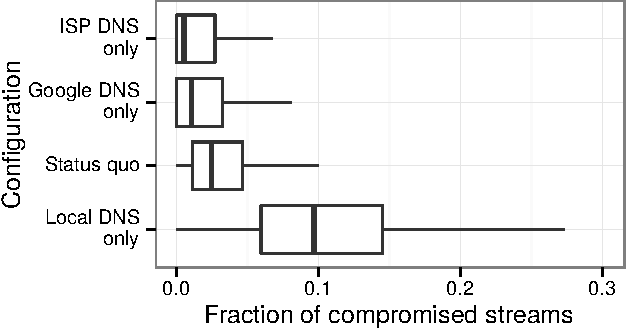
\includegraphics[width=0.75\linewidth]{figures/differences-comp-streams.pdf}
\caption{The fraction of compromised streams for the status quo and three
hypothetical DNS configurations for all exit relays (these simulated Tor users 
are in AS 7922).  
We removed outliers, so 
the box plot only shows the distributions' quartiles.  The safest configuration
is ``ISP DNS only,'' \ie have all exit relays use their ISP's DNS resolver.  The
median of compromised streams for this configuration is 0.005.}
\label{fig:compromised-streams}
\end{figure}

\begin{figure}[t]
\centering
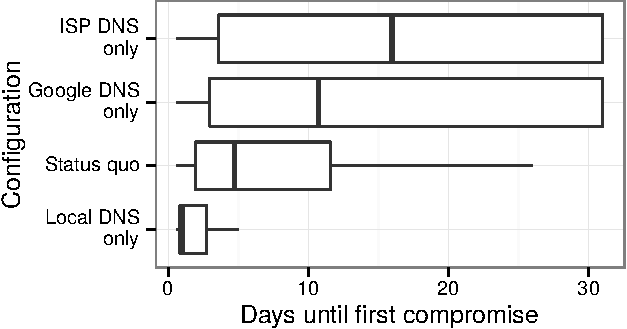
\includegraphics[width=0.75\linewidth]{figures/differences-time-comp.pdf}
\caption{The time until first stream compromise for the status quo and three
hypothetical DNS configurations for all exit relays (these simulated Tor users 
are in AS 7922).  
We removed outliers, so 
the box plot only shows the distributions' quartiles.  Again, the safest
configuration is ``ISP DNS only;'' the median of the distribution is
close to 16 days.}
\label{fig:time-until-compromise}
\end{figure}

Figures~\ref{fig:compromised-streams}
and~\ref{fig:time-until-compromise} the results of our experiments for 100,000 
simulated Tor users located in AS 7922 (United States, Comcast). (For the results 
of our experiments for users located in the other four countries, please see our Appendix. 
\emph{ISP DNS only} represents a world in which all exit relays use 
their ISPs' name servers. \emph{Google DNS only} represents a world in which all 
Tor exit relays use {\tt 8.8.8.8} for DNS resolution.  \emph{Local DNS only} represents 
a world in which all Tor exit relays perform their own DNS resolution.  And again, 
\emph{Status quo} represents our estimate of the current world of exit relay resolution.  

The figures show that \emph{ISP DNS only} fared much better than the other configurations. 
This was expected, of course, because there is only one AS (the exit relay's AS) to contend 
with on the egress side. \emph{Google DNS only} was next, and we believe this is because
of Google's heavily anycast servers. 

There is a potential tradeoff between the safety of using a well-managed 
DNS resolver such as Google's vs. a potentially not-as-well-managed 
DNS resolver from the ISP.  

Please note that the wide variance observed in Figure~\ref{fig:time-until-compromise} is 
due to using 31 days as a placeholder for sample users who were never compromised.

We believe that the \emph{Status Quo} results are significantly better than the 
\emph{Local dns only} results because only around 12\% of Tor exit relays 
actually do their own resolution. Additionally, the differing results for the 
different client ASes shows that client AS needs to be taken into account. 
